\documentclass[12pt, titlepage]{article}

\usepackage{booktabs}
\usepackage{tabularx}
\usepackage{hyperref}
\usepackage{graphics}
\usepackage{float}
\hypersetup{
    colorlinks,
    citecolor=black,
    filecolor=black,
    linkcolor=red,
    urlcolor=blue
}
\usepackage[round]{natbib}

\title{SE 3XA3: Test Plan\\Scrabble Project}

\author{214\#, The Trifecta
		\\ Kanakabha Choudhri, choudhrk
		\\ Lucia Cristiano, cristial
		\\ Raymond Tu, tur1
}

\date{February 28, 2020}

%\input{../Comments}

\begin{document}

\maketitle

\pagenumbering{roman}
\tableofcontents
\listoftables
\listoffigures

\begin{table}[bp]
\caption{\bf Revision History}
\begin{tabularx}{\textwidth}{p{3cm}p{2cm}X}
\toprule {\bf Date} & {\bf Version} & {\bf Notes}\\
\midrule
Date 1 & 1.0 & Notes\\
Date 2 & 1.1 & Notes\\
\bottomrule
\end{tabularx}
\end{table}

\newpage

\pagenumbering{arabic}

This document serves as a plan for the testing of the Scrabble Project.

\section{General Information} 

\subsection{Purpose}

The purpose of testing this project is to ensure that the system meets all the functional and non-functional requirements specified in the Software Requirements Specification.

\subsection{Scope}

The test plan contained in this document ensures all  functional and non-functional requirements are covered by tests. As well as specifying how each of the methods contained within the various software projects are to be tested for functionality and performance.

\subsection{Acronyms, Abbreviations, and Symbols}
	
\begin{table}[hbp]
\caption{\textbf{Table of Abbreviations}} \label{Table}

\begin{tabularx}{\textwidth}{p{3cm}X}
\toprule
\textbf{Abbreviation} & \textbf{Definition} \\
\midrule
SRS & Software Requirement Specification\\
GUI & Graphical User Interface\\
MIS & Module Interface Specification\\
POC & Proof of Concept \\
LF1 & Look and Feel Requirements\\
\bottomrule
\end{tabularx}

\end{table}

\begin{table}[!htbp]
\caption{\textbf{Table of Definitions}} \label{Table}
\begin{tabularx}{\textwidth}{p{3cm}X}
\toprule
\textbf{Term} & \textbf{Definition}\\
\midrule
Term1 & Definition1\\
Term2 & Definition2\\
\bottomrule
\end{tabularx}

\end{table}	

\subsection{Overview of Document}
The remainder of this document is divided into six separate sections. \\
Section two covers the overall testing plan, such as the testing team, tools being used, and the schedule for testing.\\ 
Section three breaks down the specific tests for functional and non-functional requirements and includes traceability details.\\
Section four specifies the tests used to test the construction of the proof of concept that was presented earlier on in the life of the project.\\
Section five compares the test cases included in the plan to the current implementation of the project.\\
Section six contains the details explaining and specifying the unit testing plan for the project.
Finally, section seven is an appendix that includes symbolic parameters and survey questions used elsewhere in the test plan document.

\section{Plan} 
	
\subsection{Software Description}
The software of the Scrabble project is a re-implementation of a text based version of the game that includes a GUI built using the Python library Tkinter. The inclusion of a GUI was done to make the game more accessible to a wider audience.

\subsection{Test Team}
The test team consists of the members of the Scrabble project, Kanakabha Choudhri, Lucia Cristiano, and Raymond Tu.

\subsection{Automated Testing Approach}
The scrabble project team has decided to create a set of unit tests using PyTest. These tests will test every method in the front-end and back-end for errors and ensure consistency between updates. Additionally, PyTest's inbuilt code coverage feature will also be used to measure the coverage of the unit tests. Test cases will be grouped into sections based on functional requirements and non-functional requirements. These will be broken down into tests regarding the keyboard and mouse inputs to the game. Then the back-end modules that take in this input and processes the turn will be tested. These tests will be automated and automatically ran between updates to the main branch of the repository. 

\subsection{Testing Tools} %raymond

PyTest is a framework that will be used to create unit tests for the program, as well as test for overall statement coverage in the testing approach.

\subsection{Testing Schedule} %Raymond - gantt chart
		
See Gantt Chart at the following url:

\href{https://gitlab.cas.mcmaster.ca/choudhrk/thetrifecta_scrabble/blob/master/ProjectSchedule/3XA3\%20Gantt\%20Chart.pdf}{[Click Here for Link to Gantt Chart]}

\section{System Test Description}
	
\subsection{Tests for Functional Requirements} 
Refer to Appendix Section 7.3 for explanation of omitted functional requirements one and three. 
\item{test-id1\\}

Type: 
					
Initial State: 
					
Input/Condition: 
					
Output/Result: 
					
How test will be performed: 


\subsubsection{User Input}

\paragraph{Mouse Input}

\begin{enumerate}
\item{test-UI1: Test rack size after exchanging tiles \\} %FR5
    Type: Functional, Dynamic, Manual\\
    Initial State: Player is currently on the board screen\\
    Input: The Player clicks the "Exchange Tiles" button.\\
    Output: A random tile is removed from the rack and replaced by another tile.\\
    How test will be performed: A test member will conduct a visual test to confirm that after pressing the "Exchange Tiles" button of tiles in the player's rack does not exceed $MAX\_NUM\_TILES$.

\end{enumerate}

\paragraph{Keyboard Input}
\begin{enumerate}
    \item{test-UI2: Test labels update correctly with playernames\\} %FR4
    Type: Functional, Dynamic, Manual\\
    Initial State: Player has clicked Start Game and is on the player name input screen.\\
    Input: Player inputs 2 player names, with any combination of letters and numbers.\\
    Output: Once player clicks Let's Play, player names are saved onto the board screen and outputted as titles next to player rack and player score.\\
    How test will be performed: A test member will conduct a visual test to confirm that all the labels correctly output with the player names.\\
    
    \item{test-UI3: Inputted player names only have string characters\\} %FR4
    Type: Functional, Dynamic, Manual\\
    Initial State: Player has clicked Start Game and is on the player name input screen.\\
    Input: Player inputs 2 player names, with any combination of letters and numbers.\\
    Output: Once player clicks Let's Play, player names are saved onto the board screen and outputted as titles next to player rack and player score. Player names only contain string characters.\\
    How test will be performed: A test member will conduct a visual test to confirm that all the player names only contain string characters.\\
    
    \item{test-UI4: Test rack size after turn\\} %FR5
    Type: Functional, Dynamic, Manual\\
    Initial State: Player has entered in a word, row, column and direction on the game board screen.\\
    Input: The Player clicks the "End Move" button.\\
    Output: If the word is valid the used tiles are removed from the rack and replaced with new tiles.\\
    How test will be performed: A test member will conduct a visual test to confirm that at the end of the player's turn the amount of tiles in the rack does not exceed $MAX\_NUM\_TILES$.
    
    \item{test-UI5: Test valid word\\} %FR6
    Type: Functional, Dynamic, Manual\\
    Initial State: Player has entered in a valid word, as well as row, column and direction on the game board screen.\\
    Input: The Player clicks the "End Move" button.\\
    Output: The word is placed on the game board in the correct location.\\
    How test will be performed: A test member will conduct a visual test to confirm that after pressing the "End Move" button the game board is updated with the correct word.\\ 
    
    \item{test-UI6: Test invalid length of word \\} %FR6, FR7
    Type: Functional, Dynamic, Manual\\
    Initial State: Player has entered in a word of less than $MIN\_NUM\_LETTERS$, as well as row, column and direction on the game board screen.\\
    Input: The Player clicks the "End Move" button.\\
    Output: An error label appears stating that the move is invalid.\\
    How test will be performed: A test member will conduct a visual test to confirm that after pressing the "End Move" button the error label appears and it remains that player's turn.\\
    
    \item{test-UI7: Test word not found in dictionary\\} %FR6, FR7
    Type: Functional, Dynamic, Manual\\
    Initial State: Player has entered in a word not found in the official Scrabble dictionary, as well as row, column and direction on the game board screen.\\
    Input: The Player clicks the "End Move" button.\\
    Output: An error label appears stating that the move is invalid.\\
    How test will be performed: A test member will conduct a visual test to confirm that after pressing the "End Move" button the error label appears and it remains that player's turn.\\
    
    \item{test-UI8:Test valid dimensions and direction\\} %FR8
    Type: Functional, Dynamic, Manual\\
    Initial State: Player has entered a word, valid row, valid column and valid direction on the game board screen.\\
    Input: The Player clicks the "End Move" button.\\
    Output: The word is updated on the game board in desired location and orientation.\\
    How test will be performed: A test member will conduct a visual test to confirm that after pressing the "End Move" button the starting letter of the word is at the specified row and column, as well as the word being oriented in the correct direction.\\
    
    \item{test-UI9:Test invalid row and valid direction\\} %FR8
    Type: Functional, Dynamic, Manual\\
    Initial State: Player has entered a word, invalid row, valid column and valid direction on the game board screen.\\
    Input: The Player clicks the "End Move" button.\\
    Output: An error label appears stating that the move is invalid \\
    How test will be performed: A test member will conduct a visual test to confirm that after pressing the "End Move" button the error label appears and it remains that player's turn.\\
    
    \item{test-UI10:Test invalid column and valid direction\\} %FR8
    Type: Functional, Dynamic, Manual\\
    Initial State: Player has entered a word, valid row, invalid column and valid direction on the game board screen.\\
    Input: The Player clicks the "End Move" button.\\
    Output: An error label appears stating that the move is invalid \\
    How test will be performed: A test member will conduct a visual test to confirm that after pressing the "End Move" button the error label appears and it remains that player's turn.\\
    
    \item{test-UI11:Test valid row, valid column and invalid direction\\} %FR8
    Type: Functional, Dynamic, Manual\\
    Initial State: Player has entered a word, valid row, valid column and invalid direction on the game board screen.\\
    Input: The Player clicks the "End Move" button.\\
    Output: An error label appears stating that the move is invalid \\
    How test will be performed: A test member will conduct a visual test to confirm that after pressing the "End Move" button the error label appears and it remains that player's turn.\\
    
    \item{test-UI12:Test for when the word inputted vertically forms a valid word with existing words/letters.\\} %FR9
    Type: Functional, Dynamic, Manual\\
    Initial State: Player has entered a valid word sequence, valid row, valid column and valid direction on the game board screen.\\
    Input: The Player clicks the "End Move" button.\\
    Output: The board gets updated with the new word sequence. \\
    How test will be performed: A test member will conduct a visual test to confirm that after pressing the "End Move" button the board gets updated with the valid word sequence.\\
    
    \item{test-UI13:Test for when the word inputted vertically forms an invalid word with existing word/letter.\\} %FR9
    Type: Functional, Dynamic, Manual\\
    Initial State: Player has entered an invalid word, valid row, valid column and valid direction on the game board screen.\\
    Input: The Player clicks the "End Move" button.\\
    Output: An error label appears stating that the move is invalid.\\
    How test will be performed: A test member will conduct a visual test to confirm that after pressing the "End Move" button the error label appears and it remains that player's turn.\\
    
    \item{test-UI14:Test for when the word inputted horizontally forms a valid word with existing word/letter.\\} %FR9
    Type: Functional, Dynamic, Manual\\
    Initial State: Player has entered a valid word sequence, valid row, valid column and direction on the game board screen.\\
    Input: The Player clicks the "End Move" button.\\
    Output: The board gets updated with new word sequence. \\
    How test will be performed: A test member will conduct a visual test to confirm that after pressing the "End Move" button the board gets updated with the correct word sequence.\\
    
    \item{test-UI15:Test for when the word inputted horizontally forms an invalid word with existing word/letter.\\} %FR9
    Type: Functional, Dynamic, Manual\\
    Initial State: Player has entered an invalid word sequence, valid row, valid column and valid direction on the game board screen.\\
    Input: The Player clicks the "End Move" button.\\
    Output: An error label appears stating that the move is invalid \\
    How test will be performed: A test member will conduct a visual test to confirm that after pressing the "End Move" button the error label appears and it remains that player's turn.\\
    
    \item{test-UI16:Test for standalone word score.\\} %FR10
    Type: Functional, Dynamic, Manual\\
    Initial State: The Player clicks the "End Move" button.\\
    Input: Player has entered a valid word onto the board. \\
    Output: The updated score is shown. \\
    How test will be performed: A test member will conduct a visual test to confirm that after pressing the "End Move" button the board updates players score by expected amount.\\
    
    \item{test-UI17:Test for inputted word sequence attached to existing word.\\} %FR10
    Type: Functional, Dynamic, Manual\\
    Initial State: The Player clicks the "End Move" button.\\
    Input: Player has entered a valid word sequence onto the board. \\
    Output: The updated score is shown. \\
    How test will be performed: A test member will conduct a visual test to confirm that after pressing the "End Move" button the board updates players score by expected amount.\\
    
    \item{test-UI18:Test for removal of rack when turn is finished.\\} %FR11
    Type: Functional, Dynamic, Manual\\
    Initial State: Current player's rack is visible.\\
    Input: Player clicks "End move" button. \\
    Output: The previous player's rack is replaced with the next player's rack. \\
    How test will be performed: A test member will conduct a visual test to confirm that after pressing the "End Move" button the board gets updated with a new rack.\\
    
    \item{test-UI19:Test for end game state based on allowed words.\\} %FR12
    Type: Functional, Dynamic, Manual\\
    Initial State: Board has space for one more word\\
    Input: Player clicks "End move" button. \\
    Output: The board is filled with no space for no valid words, exits and displays the highest score and the player who scored it. \\
    How test will be performed: A test member will conduct a visual test to confirm that after pressing the "End Move" button the game exits the board and displays the highest score with the player who scored that score.\\
    
    \item{test-UI20:Test for end game state based on internal bag count.\\} %FR12
    Type: Functional, Dynamic, Manual\\
    Initial State: Current bag having $N rack$ sized letters.\\
    Input: Player clicks "End move" button. \\
    Output: The internal bags size is 0 which results into game exiting board and displaying the highest score and player who scored it. \\
    How test will be performed: A test member will conduct a visual test to confirm that after pressing the "End Move" button the game exits the board and displays the highest score with the player who scored that score.\\
    
\end{enumerate}
\subsubsection{Game Environment}
\paragraph{Graphical User Interface}
\begin{enumerate}
    \item{test-GE1: Test rack size after initial board loading\\} %FR5
    Type: Functional, Dynamic, Manual\\
    Initial State: Player has entered in the two player names on the player name input screen. \\
    Input: The Player clicks the "Let's Play" button.\\
    Output: The game board screen is loaded and player one's rack is loaded with $MAX\_NUM\_TILES$.\\
    How test will be performed: A test member will conduct a visual test to confirm that player one's rack has $MAX\_NUM\_TILES$.\\
    
    \item{test-GE2: Test board size and width after initial board loading\\} %FR2
    Type: Functional, Dynamic, Manual\\
    Initial State: Player has entered in the two player names on the player name input screen. \\
    Input: The Player clicks the "Let's Play" button.\\
    Output: The game board screen is loaded with width of $BOARD\_WIDTH$ tiles and height of $BOARD\_HEIGHT$ tiles.
    How test will be performed: A test member will conduct a visual test to confirm that the game board has size of $BOARD\_WIDTHXBOARD\_HEIGHT$.\\
    
    \item{test-GE3: Test premium square locations after initial board loading\\} %FR2
    Type: Functional, Dynamic, Manual\\
    Initial State: Player has entered in the two player names on the player name input screen. \\
    Input: The Player clicks the "Let's Play" button.\\
    Output: The game board screen is loaded with coloured premium squares in the correct locations.
    How test will be performed: A test member will conduct a visual test to confirm that the game board has the premium squares in the correct locations, as well as the correct number of premium squares. Check section 7.2 for correct board layout.\\
    
    \item{test-GE4: Test score count display after valid word is entered.\\} %FR10
    Type: Functional, Dynamic, Manual\\
    Initial State: Player has entered a valid word. \\
    Input: The Player clicks the "End Move" button.\\
    Output: The game board screen section showing score gets updated with correct score.
    How test will be performed: A test member will conduct a visual test to confirm that the game board has the score section updated under correct user.\\
    
    \item{test-GE5: Test that upon arrival of the end state game exits board.\\} %FR12
    Type: Functional, Dynamic, Manual\\
    Initial State: Player is allowed to make valid moves or internal bag has $N rack$ sized amount of letters in bag. \\
    Input: The Player clicks the "End Move" button.\\
    Output: The game exits the game board to a separate screen showing player with highest score and their score.
    How test will be performed: A test member will conduct a visual test to confirm that the game board has been exited from and a new screen pops up with highest score and winner shown\\
\end{enumerate}
    
\subsection{Tests for Nonfunctional Requirements}%Raymond

\subsubsection{Look and Feel}
\begin{enumerate}

\item{test-LF1: Users find interface warm and welcoming}\\
    Type: Functional, Static, Manual\\
    Initial State: The Scrabble project game opened and loaded to the initial screen.\\
    Input/Conditions: The user takes a good look at the interface and its components.\\
    Output/Result: Most users report the user interface has a warm look and feel to it.\\
    How test will be performed: The group of testers of different personal views and opinions will statically observe the user interface and give back their opinions on what kind of impression the game gives to them.\\
\end{enumerate}

\subsubsection{Usability}
\begin{enumerate}
    \item{test-UH1: Usable by $MIN\_AGE$\\}
    Type: Functional, Dynamic, Manual\\
    Initial State: The Scrabble project game opened and loaded to the initial screen and given to user of $MIN\_AGE$ to play.\\
    Input/Conditions: The user is able to play through the game with no outside help.\\
    Output/Result:  The user will report a six or higher on the scale from one to ten when asked about their comfort playing the game. (See section 7.2)\\
    How test will be performed: The group of testers of $MIN\_AGE$ will have 85\% percent giving a rating of six or higher on the scale.\\
    
    \item{test-UH2: Test Recognizable Layout}
    Type: Functional, Dynamic, Manual\\
    Initial State: Scrabble project game is opened and loaded the initial screen and given to a user who has never played the Scrabble project.\\
    Input/Conditions: The user is able to recognize the game as Scrabble by the end of the play through.\\
    Output/Result:  The user will report a seven or higher on the scale from one to ten when asked about how recognizable the layout of the game is.(See section 7.2)\\
    How test will be performed: The group of testers will have 90\% percent giving a rating of seven or higher on the scale.\\
    
    \item{test-UH3: Test Need for Tutorial}
    Type: Functional, Dynamic, Manual\\
    Initial State: Scrabble project game is opened and loaded the initial screen and given to a user who has never played the Scrabble project game.\\
    Input/Conditions: The user is able to play through the game with no outside help and only usage of the in game instructions.\\
    Output/Result:  The user will report a seven or higher on the scale from one to ten when asked about how understandable it was to play the game. (See section 7.2)\\
    How test will be performed: The a group of testers will have 85\% percent giving a rating of seven or higher on the scale.\\
    
    \item{test-UH4: Test Previous Players}
    Type: Functional, Dynamic, Manual\\
    Initial State: Scrabble project game is opened and loaded the initial screen and given to a user who has already played a game of Scrabble.\\
    Input/Conditions: The user is able to play through the game with no outside help and not using the in game instructions.\\
    Output/Result:  The user will report a six or higher on the scale from one to ten when asked about how easy it was to remember the game. (See section 7.2)\\
    How test will be performed: The group of testers will have 90\% percent giving a rating of six or higher on the scale.\\
\end{enumerate}

\subsubsection{Performance}

\begin{enumerate}
    \item{test-PR1: Test for Turn Change Speed} %PR1
    Type: Functional, Dynamic, Manual\\
    Initial State: The player has hit the let's play button and is at the board game screen.\\
    Input/Conditions: The player inputs a valid word and move and has hit the turn change button.\\
    Output/Result:  The turn is changed and the board is updated within $MIN\_TURN\_CHANGE\_TIME$.\\
    How test will be performed: A tester will input a valid word and direction based on their rack and the game board state and hit end turn. They will visually verify that the turn changes within $MIN\_TURN\_CHANGE\_TIME$ with the correct updated board.\\
    
    \item{test-PR2: Test for Playable State Between Updates} %PR2
    Type: Functional, Dynamic, Manual\\
    Initial State: The game has been updated to the latest version. The player has hit the let's play button and is at the board game screen.\\
    Input/Conditions: The player inputs a valid word and move and has hit the turn change button.\\
    Output/Result:  The turn is changed and the board is updated correctly.\\
    How test will be performed: A tester will input a valid word and direction based on their rack and the game board state and hit end turn. They will visually verify that the game is in a playable state, ie. turn changes in a reasonable amount of time with the correct updated board. Additionally, a questionnaire will be provided to a sample set of users and at least 90\% will confirm software is playable prior to the next update.\\
\end{enumerate}

\subsubsection{Operational and Environmental}
\begin{enumerate}

\item{test-OE1: The Scrabble game takes no more than 20 minutes to install onto the host computer.}\\
    Type: Functional, Dynamic, Manual\\ %OE1
    Initial State: User has the link necessary for downloading the game.\\
    Input/Conditions: The user follows necessary steps to download the game.\\
    Output/Result: The game has been downloaded and stored into correct folder within 20 minutes of initializing download. \\
    How test will be performed: The group of testers with different kinds of PC's will download the game and note how long it took them to download it and set it up on their PC's.\\
    
\item{test-OE2: The Scrabble game takes no more than 10 seconds to load.}\\
    Type: Functional, Dynamic, Manual\\ %OE2
    Initial State: User has downloaded the game.\\
    Input/Conditions: User tries to open the game.\\
    Output/Result: Users note that the game doesn't take too long(more than 10 seconds) to load. \\
    How test will be performed: The group of testers having the game installed on their PC will try to load the game and note how long it took them to do so.\\
    
\end{enumerate}

\subsubsection{Maintainability and Support}

\begin{enumerate}
    \item{test-MS1: Test for Maintainability} %MS1 - kinda weird
    Type: Functional, Dynamic, Manual\\
    Initial State: The source code has been reviewed by a focus group of programmers.\\
    Input/Conditions: The source code of the repository.\\
    Output/Result:  The maintainability of the system is rated from 1-5.\\
    How test will be performed: A focus group of programmers will do a code review of the source code of the game. They will rate the maintainability of the game for future updates between 1-5. For the test case to pass, the average score of maintainability must be higher than 4.\\
    
    \item{test-MS2: Test for Implementation of New Features} %MS2
    Type: Functional, Dynamic, Manual\\
    Initial State: The source code has been reviewed by a focus group of programmers.\\
    Input/Conditions: The source code of the repository.\\
    Output/Result:  The maintainability of the system is rated on a scale from 1-10.\\
    How test will be performed: A focus group of software design experts will do a code review of the source code of the game. They will rate how modular the game is and if it allows for easy implementation of new features, on a scale from 1-10. For the test case to pass, the average score must be higher than 4=8.\\
    
    \item{test-MS3: Test for Playable State Between Python Updates} %MS3
    Type: Functional, Dynamic, Manual\\
    Initial State: The game has been updated to the latest version on Github. The player's system has been updated to the latest version of Python 3. The player has hit the let's play button and is at the board game screen.\\
    Input/Conditions: The player inputs a valid word and move and has hit the turn change button.\\
    Output/Result:  The turn is changed and the board is updated correctly.\\
    How test will be performed: A tester will input a valid word and direction based on their rack and the game board state and hit end turn. They will visually verify that the game is in a playable state, ie. turn changes in a reasonable amount of time with the correct updated board. Additionally, a questionnaire will be provided to a sample set of users and the average score from 1-10 must be at least an 8.\\
\end{enumerate}

\subsection{Traceability Between Test Cases and Requirements}%Lucia
\begin{table}[H]
  \begin{center}
    \caption{Traceability for Functional Requirements}
    \label{tab:table1}
    \begin{tabular}{c|c} 
        \toprule
        \textbf{Functional Requirement} & \textbf{Test Cases}\\
        \midrule
        FR2 & test-GE1, test-GE2\\
        \hline
        FR4 & test-UI2, test-UI3\\
        \hline
        FR5 & test-UI1, test-UI4, test-GE1\\
        \hline
        FR6 & test-UI5, test-UI6\\
        \hline
        FR7 & test-UI6, test-UI7\\
        \hline
        FR8 & test-UI8, test-UI9, test-UI10, test-UI11\\
        \hline
        FR9 &  test-UI12, test-UI13, test-UI14, test-UI15\\
        \hline
        FR10 & test-UI16, test-UI17, test-GE4\\
        \hline
        FR11 & test-UI18\\
        \hline
        FR12 & test-UI19, test-UI20, test-GE5\\
        \bottomrule
    \end{tabular}
  \end{center}
\end{table}

\begin{table}[H]
  \begin{center}
    \caption{Traceability for Non-Functional Requirements}
    \label{tab:table1}
    \begin{tabular}{c|c} 
        \toprule
        \textbf{Non-Functional Requirement} & \textbf{Test Cases}\\
        \midrule
        NFR LF1 & test-LF1 \\
        \hline
        NFR UH1 & test-UH1\\
        \hline
        NFR UH2 & test-UH2\\
        \hline
        NFR UH4 & test-UI3\\
        \hline
        NFR UH5 & test-UH4\\
        \hline
        NFR PR1 & test-PR1\\
        \hline
        NFR PR2 & test-PR2\\
        \hline
        NFR OE1 & test-OE1 \\
        \hline
        NFR OE2 & test-OE2 \\
        \hline
        NFR MS1 & test-MS1\\
        \hline
        NFR MS2 & test-MS2\\
        \hline
        NFR MS3 & test-MS3 \\
        \bottomrule
    \end{tabular}
  \end{center}
\end{table}

\section{Tests for Proof of Concept}%Raymond
Proof of Concept testing is similar to the planned testing above of the actual game implementation, although missing many features regarding the functionality of the game. The goal of the proof of concept was to create the GUI of the game in Tkinter to demonstrate it's feasibility. Therefore, all of the tests will be strictly regarding the front end of the game. 

\subsection{Board Layout}

Testing for the board layout will ensure the size of the game board and the layout of the premium is correct (See Section 7.2 Figure 1 for correct board layout). Additionally, the overall aesthetic appeal of the POC and it's visual similarity to the scrabble game will be tested. See (test-GE1, test-GE2) for testing the board size and layout of premium squares. See (test-LF1) for testing the aesthetic appeal of the POC. 

\subsection{Label Layout}

Testing for the label layout will ensure the labels to the right of the board fit on the screen (See Section 7.2) and are in the correct layout. Additionally, the testing will ensure that player names are correctly appended to the labels. See (test-UI2, test-UI3) for testing whether player names are correctly updated. See below test cases for testing the correct label output.

\begin{enumerate}
    \item{test-POC1: Test Label Layout\\} 
    Type: Functional, Dynamic, Manual\\
    Initial State: Player has entered in the two player names on the player name input screen. \\
    Input: The Player clicks the "Let's Play" button.\\
    Output: The game board screen is loaded with correct label layout and button layout. All labels and buttons fit in the window.
    How test will be performed: A test member will conduct a visual test to confirm that the label and button layout is correct, and that all buttons and labels fit within the window margins. Check section 7.2 for the correct board layout.\\
\end{enumerate}
	
\section{Comparison to Existing Implementation}	%Lucia
When writing tests for the Scrabble project the team considered how recognizable this digital version of the game is to the board game version of Scrabble. This can be seen in test-UH2 which surveys users who played the game about their ability to recognize the GUI of the Scrabble project as the board game Scrabble.\\
Another test that takes the existing implementation into consideration is having a user that has already played Scrabble before testing how easy it is to remember how to play the game. This test can be seen in test-UH4.
\section{Unit Testing Plan}%Lucia
For unit testing of the Scrabble project PyTest will be used to write the test suites as well as determine coverage of the methods and classes being tested. 
\subsection{Unit testing of internal functions}
Unit testing of the project will consist of testing each of the modules individually by creating test cases for each of the major methods within the module. Using PyTest, test cases will be written that  compare the actual output of the methods to the expected output of the method. The tests will also check if exceptions in the method are handled in the correct manner. These tests are intended to ensure that the entire module and its methods function as outlined in the SRS and the MIS.\\
The unit testing step is crucial, as the modules must function as intended before proceeding to perform integration testing. Since the Scrabble project is a game all the modules work together to ensure that the game runs as intended. This testing step cannot be completed unless unit testing is done thoroughly.
		
\subsection{Unit testing of output files}	
The Scrabble project does not contain any explicit output files, however, it does have a GUI that outputs to the screen of the machine the game is being played on. The testing of this interface will be completed based on the tests for functional requirements. These tests involve passing in a certain input from the mouse and keyboard and rely on visual confirmation that the GUI has outputted the correct results. This type of manual testing is necessary to ensure that the outputs of the project are sensible and result in a playable game.


\bibliographystyle{plainnat}

\bibliography{}

\newpage

\section{Appendix}

Additional information included here.

\subsection{Symbolic Parameters}
% The definition of the test cases will call for SYMBOLIC\_CONSTANTS.
% Their values are defined in this section for easy maintenance.
$MAX\_NUM\_TILES= 7$\\
$MIN\_NUM\_LETTERS = 2$\\
$MIN\_AGE = 8$\\
$BOARD\_WIDTH$ = 15\\
$BOARD\_HEIGHT$ = 15\\
$MIN\_TURN\_CHANGE\_TIME$ = 10 seconds\\
$N$ = How many letters are supposed to go in one rack\\

\subsection{Figures}

\begin{figure}[H]
    \centering
    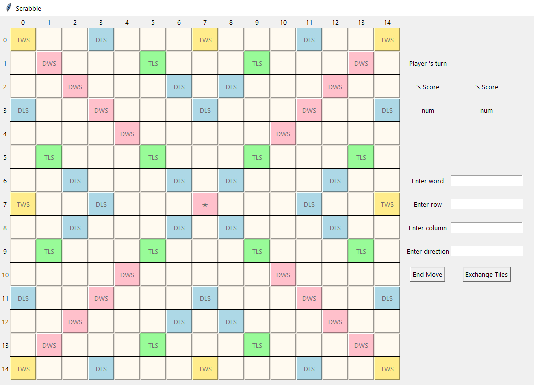
\includegraphics{TestPlan/Scrabble Board.png}
    \caption{Board Layout}
    \label{fig:my_label}
\end{figure}

\subsection{Removed Functional Requirements}
Functional Requirements one and three were deemed obsolete based on feedback on the SRS document and decisions made by the Scrabble project team. Since these requirements have been removed there are not any test cases written for them.\\
\subsection{Usability Survey Questions}
For test-UH1: How comfortable on a scale of 1-10 were you with playing the Scrabble game?\\
For test-UH2: How easy was it to identify this game as Scrabble on a scale of 1-10?\\
For test-UH3: How easy was it to play the game without a tutorial on a scale of 1-10?\\
For test-UH4: How easy was it to remember how to play the game on a scale of 1-10?\\
For test-PR2: Can you confirm the game is playable after the latest update (Yes/No)?\\
For test-MS1: How maintainable is the game for future updates on a scale of 1-5?\\
For test-MS2: How easily can new features be added to the game on a scale of 1-10?\\
For test-MS3: How would you rate the playability of the game after the latest Python 3 update on a scale of 1-10?\\
% This is a section that would be appropriate for some teams.

\end{document}